\documentclass[a4paper, 12pt]{article}

\usepackage[dvipsnames]{xcolor} % Code highlighting color
\usepackage[catalan]{babel} % Language 
\usepackage{fontspec} 
\usepackage{fullpage}
\usepackage[a4paper, margin=2cm]{geometry} % To change the margins
\usepackage{graphicx} % Insert images
\usepackage[hidelinks]{hyperref} % Links color
\usepackage[final]{pdfpages}
\usepackage{ragged2e}
\usepackage{wrapfig} %To Text wrap
\usepackage{listings} % Add code
\usepackage{verbatim}
\usepackage{tikz}
\usepackage{subcaption}
\usepackage{multirow}
\usepackage{colortbl}


\usetikzlibrary{arrows, positioning, shapes}

\tikzstyle{vec1} = [rectangle, centered, draw, minimum height = .8cm, minimum width=2.2cm]
\tikzstyle{vec2} = [vec1, minimum width=1.8cm]
\tikzstyle{arrow} = [thick,->,>=stealth]
\tikzstyle{scat} = [ scale=0.8, every node/.style={scale=0.8} ]

\renewcommand*\contentsname{Índex}
\setlength\parindent{0pt}

\lstset{ %
	backgroundcolor=\color{white},   % choose the background color; you must add \usepackage{color} or \usepackage{xcolor}
	basicstyle=\footnotesize,        % the size of the fonts that are used for the code
	captionpos=b,                    % sets the caption-position to bottom
	extendedchars=true,              % lets you use non-ASCII characters; for 8-bits encodings only, does not work with UTF-8
	keepspaces=true,                 % keeps spaces in text, useful for keeping indentation of code (possibly needs columns=flexible)
	keywordstyle=\color{blue},       % keyword style
	numbers=none,                    % where to put the line-numbers; possible values are (none, left, right)
	rulecolor=\color{black},         % if not set, the frame-color may be changed on line-breaks within not-black text (e.g. comments (green here))
	showspaces=false,                % show spaces everywhere adding particular underscores; it overrides 'showstringspaces'
	showstringspaces=false,          % underline spaces within strings only
	showtabs=false,                  % show tabs within strings adding particular underscores
	tabsize=2,	                   % sets default tabsize to 2 spaces
}

\begin{document}
\title{\textsc{Cerca local}}
\author{Marc Asenjo i Ponce de León \and
	Joan Marcè i Igual \and
	Iñigo Moreno i Caireta}
\date{\today}
\maketitle

\section{Implementació estat}
La nostra implementació d'estat utilitza dos vectors de 2 dimensions. Un conté els fitxers que ha demanat cada usuari i l'altre vector, el servidor que serveix aquest fitxer. Així doncs al modificar l'estat només es modifica el segon vector permetent que el primer sigui una variable \verb|static|.

\begin{figure}[ht]
\centering
\begin{minipage}[t]{0.49\textwidth}
\begin{tikzpicture}[auto, align=center, node distance = 0cm, scat]

\node(U1)[vec1] {Usuari 1};
\node(U2)[vec1, right = of U1] {Usuari 2};
\node(U3)[vec1, right = of U2, minimum width = 3cm] { ... };
\node(U4)[vec1, right = of U3] {Usuari n};

\node(F1)[vec2, below = of U1, yshift=-1cm]{Arxiu 1};
\node(F2)[vec2, below = of F1]{Arxiu 2};
\node(F3)[vec2, below = of F2]{...};
\node(F4)[vec2, below = of F3]{Arxiu n};

\node(F5)[vec2, below = of U2, yshift=-1cm]{Arxiu 1};
\node(F6)[vec2, below = of F5]{Arxiu 3};
\node(F7)[vec2, below = of F6]{Arxiu m};

\draw [arrow] (U1) -- (F1);
\draw [arrow] (U2) -- (F5);

\end{tikzpicture}
\caption{Representació del vector de fitxers so\l.licitats per cada petició}
\end{minipage}
\hfill
\begin{minipage}[t]{0.49\textwidth}
\begin{tikzpicture}[auto, align=center, node distance = 0cm, scat]

\node(U1)[vec1] {Usuari 1};
\node(U2)[vec1, right = of U1] {Usuari 2};
\node(U3)[vec1, right = of U2, minimum width = 3cm] { ... };
\node(U4)[vec1, right = of U3] {Usuari n};

\node(F1)[vec2, below = of U1, yshift=-1cm]{Serv 7};
\node(F2)[vec2, below = of F1]{Serv 4};
\node(F3)[vec2, below = of F2]{...};
\node(F4)[vec2, below = of F3]{Serv n};

\node(F5)[vec2, below = of U2, yshift=-1cm]{Serv 2};
\node(F6)[vec2, below = of F5]{Serv 3};
\node(F7)[vec2, below = of F6]{Serv m};

\draw [arrow] (U1) -- (F1);
\draw [arrow] (U2) -- (F5);

\end{tikzpicture}
\caption{Representació del vector dels servidors assignats a cada petició}
\end{minipage}
\end{figure}

\section{Operadors}

S'han  creat dos operadors diferents, tots dos basats en el mateix principi. El primer operador (1)
canvia el servidor que serveix una petició. Donats un identificador
de usuari (\verb|uid|), una petició (\verb|rid|) i un servidor (\verb|sid|). Assigna el servidor \verb|sid|
perquè envii la petició \verb|rid|.

\begin{lstlisting}[language=java ]
public void swapServer(int uid, int rid, int sid);
\end{lstlisting}

El segon operador (2) és igual que el primer però aplicant-ho dos cops de manera que es canvien els servidors 
assignats a dues peticions. Això permet generar successors molt diferents els uns dels altres de manera que
(en teoria) es poden trobar més solucions tot i que el temps d'execució és més elevat.

\section{Estratègies solució inicial}
S'han plantejat dues estratègies generadores de la solució inicial, la primera, per cada petició, assigna
un servidor aleatori que contingui el fitxer demanat; la segona, assigna a cada petició el servidor amb menys
temps de transmissió per aquesta petició. 


\section{Funcions heurístiques}
Tal i com s'explica a l'enunciat s'han de crear dos heurístics, un per tal de minimitzar el temps del servidor
que necessita més temps per transmetre les seves peticions i un altre per minimitzar el temps total de transmissió 
però amb un temps per servidor el més similar possible entre tots els servidors.

Pel primer heurístic s'ha agafat com a valor de l'heurístic el valor de temps del servidor que triga més.

Pel segon heurístic s'ha agafat com a valor de l'heurístic la següent fórmula sobre el conjunt de dades dels temps
de transmissió de cada servidor.
$$\mu\cdot\overline{x}^2 + \sigma^2$$
On $\sigma$ és la variància, $\overline{x}$ és la mitjana i $\mu$ és un factor que s'ha d'escollir experimentalment.

\section{Experiments}
\subsection{}
Es demana escollir el conjunt d'operadors que dóna millors resultats per a la funció heurística que optimitzi el 
primer criteri. Per obtenir els resultats s'han utilitzat 10 llavors diferents, han estat les mateixes 10 tant per l'operador 1 
com pel 2. Als resultats es pot veure que les solucions dels operadors 1 i 2 són molt semblants, la solució
obtinguda amb l'operador 2 és millor però en canvi el temps per trobar la solució és tant gran que ni tan sols s'aprecia
al gràfic pel que s'acaba escollint l'operador 1.

\begin{figure}[h]
\centering
\begin{minipage}[t]{0.48\textwidth}
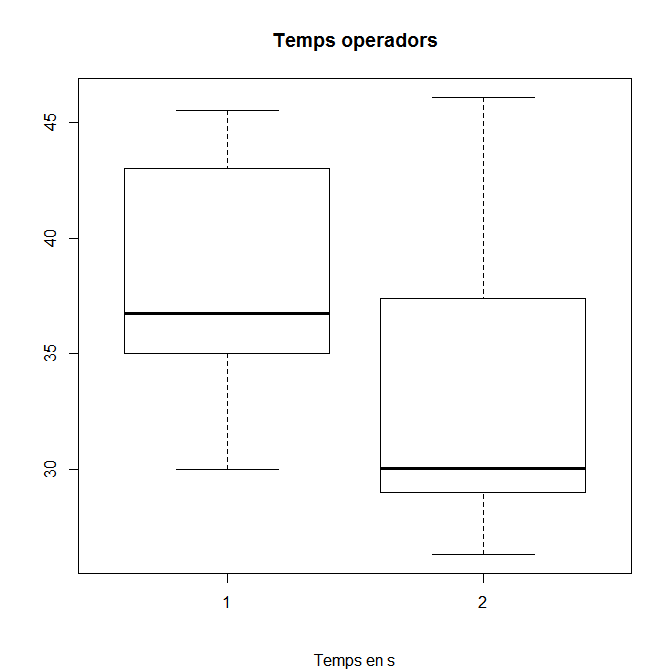
\includegraphics[width=\linewidth]{operadors}
\caption{Box plot dels temps màxims dels resultats al utilitzar l'operador 1 i 2}
\end{minipage}
\hfill
\begin{minipage}[t]{0.48\textwidth}
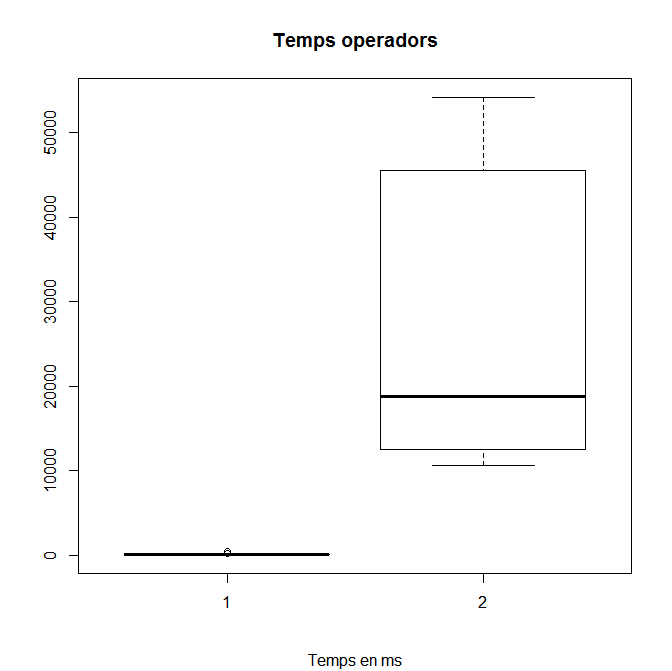
\includegraphics[width=\linewidth]{operadorsT}
\caption{Box plot dels temps que es triga en calcular la solució amb els operadors 1 i 2}
\end{minipage}
\end{figure}

\begin{table}[h!]
\begin{tabular}{l | l || l | l}
	\multicolumn{2}{c||}{Operador 1} & \multicolumn{2}{|c}{Operador 2} \\
	\hline
	Resultat (s) & Temps (ms) & Resultat (s) & Temps (ms) \\
	\hline
	35 & 415 & 30 & 45.523 \\
	41 & 110 & 29 & 54.225 \\
	35 & 168 & 37,4 & 16.391 \\
	35,5 & 104 & 34 & 11.272 \\
	45,5 & 81	& 46,1 & 10.543 \\
	35,5 & 91 & 30,1 & 15.442 \\
	43 & 33 & 28,4 & 34.781 \\
	30 & 89 & 29,9 & 21.260 \\
	38 & 53 & 40,3 & 12.497 \\
	44 & 79 & 26,3 & 47.050 \\
\end{tabular}
\caption{Resultats i temps obtinguts amb els operadors 1 i 2}
\end{table}

\newpage
\subsection{}
Es demana comparar l'estratègia de generació de la solució inicial amb els criteris de l'apartat anterior. També s'han utilitzat 10
llavors diferents per obtenir els paràmetres inicials. 

\begin{minipage}{\textwidth}
\centering
\begin{minipage}[b]{0.55\linewidth}
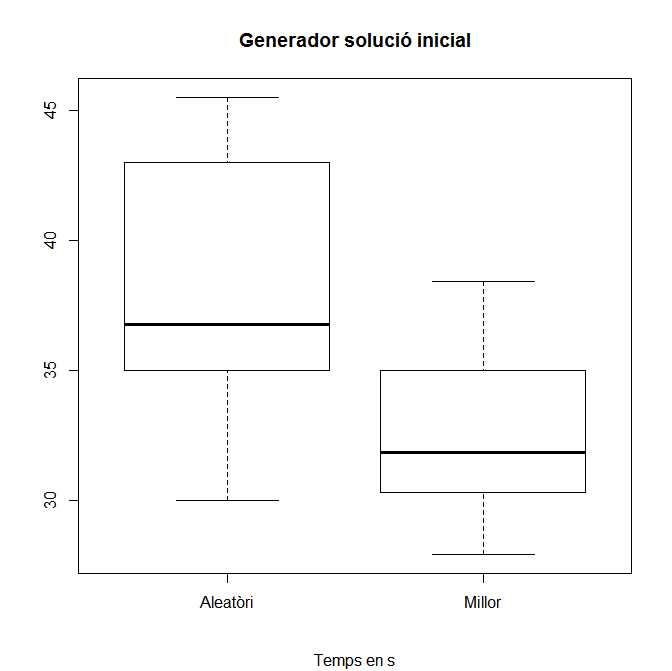
\includegraphics[width=\linewidth]{generador}
\captionof{figure}{Box plot dels temps màxims dels resultats}
\end{minipage}
\hfill
\begin{minipage}[b]{0.34\linewidth}
	\centering
	\begin{tabular}{l || l}
		Aleatori & Millor servidor \\
		\hline
		35 & 32,8 \\
		41 & 35,6 \\
		35 & 32,4 \\
		25,5 & 30,3 \\
		45,5 & 38,4 \\
		35,5 & 29,7 \\
		43 & 35 \\
		30 & 27,9 \\
		38 & 30,6 \\ 
		44 & 31,3 \\
	\end{tabular}
	\captionof{table}{Resultats (en segons) dels dos algoritmes de generació}
\end{minipage}
\end{minipage}

\newpage
\subsection{}
En aquest experiment s'han de trobar els paràmetres que donaran un millor resultat al Simulated Annealing
per l'heurístic 1. Per fer-ho es busca exhaustivament els valors de $\lambda$ i $k$ mantenint constants el
nombre d'iteracions i passos per canvi de temperatura. S'ha decidit establir aquests valors a 20.000 i 20 
respectivament ja que amb aquests valors es troben bons resultats en un temps d'execució
relativament petit. La cerca dels valors de $\lambda$ i $k$ ha seguit el següent patró:

Primer s'ha escollit valors de $\lambda$ i $k$ molt extrems per veure quins ordres de magnitud donaven uns
resultats millors: $k=\{1,1e6; 1e12\}$ i $\lambda=\{1e-5; 0,01; 1\}$. El millor d'aquests resultats ha estat
${ k = 1; \lambda = 0,01 }$.

Tot seguit s'han acotat millor els resultats, tornant a repetir l'experiment amb $k=\{1,1e2; 1e4\}$ i 
$\lambda=\{ 0,001; 0,01; 0,1 \} $. Dels resultats d'aquest experiment es pot observar que els valors on
$\lambda = 0,1$ i $k = 1e4$ són significativament més alts que la resta, però els altres són molt similars.

Finalment s'acaben d'acotar els valors repetint l'experiment amb $k=\{1; 10; 100\}$ i $\lambda=\{0,001; 0,03; 0,01\}$.
Novament es veu que els resultats són molt similars, així que es decideix parar aquí i agafar com a millors
paràmetres els valors $k=10$ i $\lambda = 0,03$.


\begin{minipage}{\linewidth}
	\begin{minipage}[b]{0.33\linewidth}
		\scriptsize
		\centering
		\begin{tabular}{l | l | l | l | l|}
			\multicolumn{1}{c}{} & \multicolumn{4}{c}{$\lambda$} \\
			\cline{3-5}
			\multicolumn{2}{c|}{} & 0,0001 & 0,01 & 1 \\
			\cline{2-5}
			\multirow{3}{*}{$k$}
			& 1 & \cellcolor{Green} 25.506 & \cellcolor{Green} 25.497 &\cellcolor{Red!60} 44.943 \\
			& 1e6 & \cellcolor{Goldenrod!70}42.973 & \cellcolor{Green} 25.651 & \cellcolor{Red!30}43.790\\
			& 1e12 & \cellcolor{Goldenrod!60}42.337 & \cellcolor{Green}25.998 & \cellcolor{Red}45.401 \\
			\cline{2-5}
		\end{tabular}
		\captionof{table}{Primer experiment}
	\end{minipage}
	\hfill
	\begin{minipage}[b]{0.32\linewidth}
		\scriptsize
		\centering
		\begin{tabular}{l | l | l | l | l|}
			\multicolumn{1}{c}{} & \multicolumn{4}{c}{$\lambda$} \\
			\cline{3-5}
			\multicolumn{2}{c|}{} & 0,001 & 0,01 & 0,1 \\
			\cline{2-5}
			\multirow{3}{*}{$k$}
			& 1 & \cellcolor{Green!50} 25.610 & \cellcolor{Green} 25.497 & \cellcolor{Red!60}30.733 \\
			& 1e2 & \cellcolor{Goldenrod!70}25.867 & \cellcolor{Green!60}25.577 & \cellcolor{Red!60}30.788 \\
			& 1e4 & \cellcolor{Goldenrod}26.666 & \cellcolor{Green!40}25.715 & \cellcolor{Red!60}30.474 \\
			\cline{2-5}
		\end{tabular}
		\captionof{table}{Segon experiment}
	\end{minipage}
	\hfill
	\begin{minipage}[b]{0.33\linewidth}
		\scriptsize
		\centering
		\begin{tabular}{l | l | l | l | l|}
			\multicolumn{1}{c}{} & \multicolumn{4}{c}{$\lambda$} \\
			\cline{3-5}
			\multicolumn{2}{c|}{} & 0,001 & 0,03 & 0,01 \\
			\cline{2-5}
			\multirow{3}{*}{$k$}
			& 1 & \cellcolor{Goldenrod!60} 25.610 & \cellcolor{Red!60} 25.745 &\cellcolor{Green!40} 25.497 \\
			& 10 & \cellcolor{Goldenrod!70}25.867 & \cellcolor{Red!40} 25.677 & \cellcolor{Green!60}25.577 \\
			& 100 & \cellcolor{Red}26.666 & \cellcolor{Green}25.446 & \cellcolor{Goldenrod!60}25.715 \\
			\cline{2-5}
		\end{tabular}
		\captionof{table}{Tercer experiment}
	\end{minipage}
\end{minipage}

\vspace{1cm}

% Pregunta 4
\subsection{}

Ara s-ha de trobar com afecta la mida del problema al temps d'execució del Hill Climbing. Primer es mirarà com afecta 
el nombre de usuaris i després també, el de servidors. En el primer gràfic es pot veure el temps d'execució del programa 
amb 50 servidors i usuaris entre 100 i 2000. Es pot veure que la funció s'assembla bastant a una quadràtica. Això és degut
a què el nombre d'usuaris fa que augmenti el factor de ramificació del problema i també fa que calgui fer més moviments 
per arribar a la solució final del Hill Climbing. Es troba una corba
de tendència exponencial $ y = 134,22e^{0,0021x} $.

\vspace{1cm}

\begin{minipage}[b]{\linewidth}
	\centering
	\begin{minipage}[b]{0.68\linewidth}
		\centering
		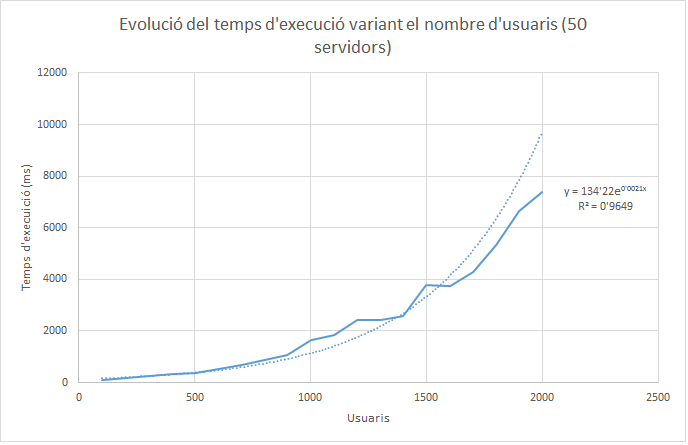
\includegraphics[width=\linewidth]{Exercici4.1}
		\captionof{figure}{Gràfic amb els temps d'execució en funció dels usuaris}
	\end{minipage}
	\hfill
	\begin{minipage}[b]{0.3\linewidth}
	\scriptsize
	\centering
	\begin{tabular}{l | l}
	Usuaris & Temps (ms) \\
	\hline
	100 & 83,3 \\
	200 & 173,7 \\
	300 & 265,2 \\
	400 & 337,3 \\
	500 & 374,1 \\
	600 & 539,2 \\
	700 & 689,9 \\
	800 & 874,8 \\
	900 & 1.076,2 \\
	1000 & 1.666,5 \\
	1100 & 1.835,8 \\
	1200 & 2.407,3 \\
	1300 & 2.430,9 \\
	1400 &	2.588,20 \\
	1500 &	3.776,20\\
	1600 &	3.741,00\\
	1700 &	4.285,30\\
	1800 &	5.315,80\\
	1900 &	6.639,50\\
	2000 &	7.395,50\\
	\end{tabular}
	\captionof{table}{Usuaris - Temps}
	\end{minipage}
\end{minipage}
\vspace{1cm}

En el segon gràfic es pot veure que el temps d'execució del programa amb 200 usuaris disminueix a mesura que s'afegeixen més 
servidors. Això es degut a una optimització que fa la funció de successió quan s'usa l'heurístic 1. Com que només es té en 
compte el temps del servidor més ocupat, movent una única petició de servidor s'aconsegueix disminuir el valor de l'heurístic
si la petició l'estava servint el servidor més ocupat. Per tant, la funció de successió només afegeix a la llista de possibles 
successors aquest tipus de moviments. Amb aquesta optimització es pot veure que el factor de ramificació no augmenta amb el 
nombre de servidors, sinó que disminueix, ja que el servidor més ocupat tindrà menys peticions. Es troba una corba de tendència
$ y = -45,69ln(x) + 354,32 $

\vspace{1cm}

\begin{minipage}[b]{\linewidth}
	\begin{minipage}[b]{0.69\linewidth}
		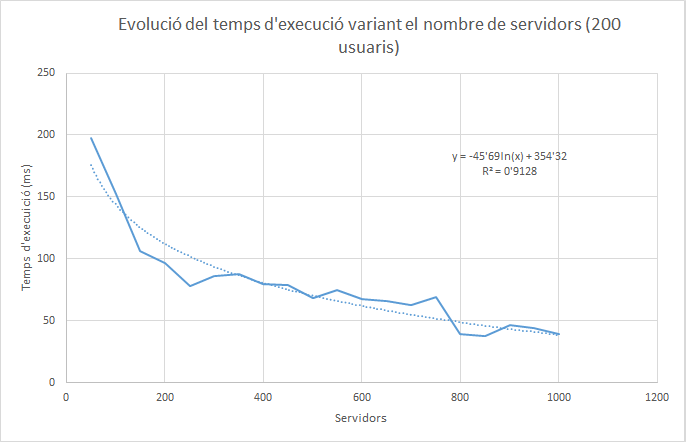
\includegraphics[width=\linewidth]{Exercici4.2}
		\captionof{figure}{Gràfic amb el temps d'execució en funció dels servidors}
	\end{minipage}
	\hfill
	\begin{minipage}[b]{0.3\linewidth}
		\scriptsize
		\begin{tabular}{l | l}
			Servidors & Temps \\
			\hline
			50	& 197,9 \\
			100	& 152,2 \\
			150	& 106,3 \\
			200	& 97 \\
			250	& 78,2 \\
			300	& 86 \\
			350	& 87,4 \\
			400	& 79,70 \\
			450	& 79,10 \\
			500	& 68,30 \\
			550	& 74,50 \\
			600	& 67,60 \\
			650	& 65,60 \\
			700	& 62,70 \\
			750	& 68,80 \\
			800	& 39,10 \\
			850	& 37,40 \\
			900	& 46,40 \\
			950	& 44,00 \\
			1000	& 39,10 \\
		\end{tabular}
		\captionof{table}{Servidors - Temps}
	\end{minipage}
\end{minipage}

\subsection{}
En aquest apartat es demana la diferència entre el temps de càlcul de la solució i el temps de 
transmissió total del resultat pels dos heurístics. Per obtenir aquests valors s'han fet 10
execucions amb llavors diferents per cada heurístic.
Així doncs pel primer heurístic s'ha obtingut de mitjana $\overline{x} = 1.457.671 s$ de diferència
entre el temps total i el de càlcul, això representa un $0,005\%$ del temps total. Pel segon
heurístic s'ha obtingut de mitjana $\overline{x} = 480.236 s$ de diferència entre els dos temps,
representant així un $1,36\%$ del temps total.
Com es pot observar, l'heurístic 2 és el que triga un percentatge més alt del temps total de transmissió
a donar la solució tot i així aquest percentatge és bastant petit i la solució trobada és molt millor.

\begin{table}[h!]
\begin{tabular}{l | l | l || l | l | l}
	\multicolumn{3}{c||}{Heurístic 1} & \multicolumn{3}{c}{Heurístic 2} \\
	\hline
	Transmissió & Càlcul & Diferència & Temps Transmissió & Temps Càlcul & Diferència \\
	\hline
	1.470.205 &	186,4&	1.470.019&	503.998	& 7608,5&	496.390 \\
	1.566.881&	185,2&	1.566.696&	517.399&	7370&	510.029 \\
	1.509.443&	77,8&	1.509.365&	462.998&	6491&	456.507 \\
	1.398.426&	47,2&	1.398.379&	481.014&	5958&	475.056 \\
	1.519.400&	36	&1.519.364	& 509.893&	6571&	503.322 \\
	1.368.733&	50,8&	1.368.682&	462.345&	5694&	456.651 \\
	1.446.608&	20	&1.446.588	& 484.512&	6431&	478.081 \\
	1.351.137&	63	&1.351.074	& 457.649&	6089&	451.560 \\
	1.449.413&	64,8&	1.449.348&	513.346&	7325&	506.021 \\
	1.497.250&	50,4&	1.497.200&	475.598&	6856&	468.742 \\
\end{tabular}
\caption{Temps de càlcul, de transmissió i diferència respecte la solució}
\end{table}

En aquest apartat ha aparegut per primer cop el segon heurístic, el que busca minimitzar el 
temps total de transmissió però intentant també mantenir els temps dels servidors per
separat el màxim de semblants possible. Com que en aquest cas hi ha més d'un factor a tenir en compte
per l'heurístic, s'ha hagut de buscar els paràmetres que s'ajusten millor al que es vol a l'hora de 
calcular l'heurístic. 
Per trobar la funció heurística adequada al que es vol optimitzar, s'ha pensat que el millor és separar-la
en dues parts. La primera serà la mitjana del temps de transmissió entre tots els servidors, és el primer
element que es vol minimitzar. La segona ha de reflectir si els temps dels servidors són molt diferents
entre ells o no, per això, s'ha escollit la variància com a mesura.

En un principi hi va haver el dubte sobre si elevar al quadrat o no la mitjana, però si no ses feia
la variància era simplement massa dominant en l'heurístic, així que la funció final és la següent:
$$\mu\cdot\overline{x}^2 + \sigma^2$$

On $\sigma$ és la variància, $\overline{x}$ és la mitjana i $\mu$ és un factor que s'ha d'escollir experimentalment.
Per tal de trobar el factor que multiplica a la mitjana s'han provat els següents valors:

\begin{table}[h]
\centering
\footnotesize
\begin{tabular}{l | l}
	Factor & Temps total de transmissió \\
0&	1.524.629 \\
1&	1.405.788 \\
2&	1.168.544 \\
3&	938.895 \\
4&	777.606 \\
5&	680.148 \\
6&	619.330 \\
7&	575.850 \\
8&	555.613 \\
9&	536.870 \\
10&	524.984 \\
20&	486.875 \\
30&	480.912 \\
50&	476.062 \\
\end{tabular}
\caption{Taula amb el valor usat del factor i el temps total de transmissió obtingut}
\end{table}

\newpage
\subsection{}

En la taula es pot veure que el HC triga molt mes quan fa servir el heurístic 2 pero que es el que troba resultats millors. El simulated annealing es molt mes ràpid i casi arriba als mateixos resultats.
\begin{table}[h]
\begin{minipage}[b]{0.49\linewidth}
	\centering
\begin{tabular}{l|l|l}
&	SA&	HC \\
\hline
	h1&	925'6&	124'1\\
	h2&	521'7&	6763'3\\
\end{tabular}
\end{minipage}
\hfill
\begin{minipage}[b]{0.49\linewidth}
	\centering
\begin{tabular}{l|l|l}
	& SA &	HC \\
	\hline
	h1	& 1.145.655,60&	1.453.201 \\
	h2	& 526.029,00&	483.024  \\
\end{tabular}
\end{minipage}
\end{table}

\subsection{}
En aquest exercici es demana l'evolució del temps d'execució i el temps total de transmissió en funció del
nombre de replicacions pels dos heurístics.

\begin{figure}[h!]
\begin{minipage}[b]{0.49\linewidth}
	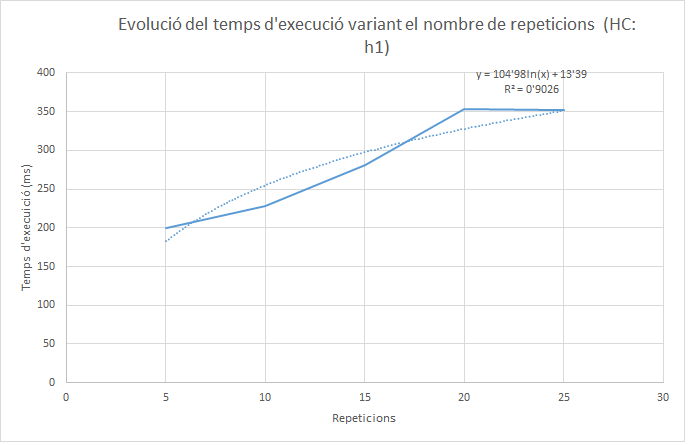
\includegraphics[width=\linewidth]{Exercici7.1.1}
\end{minipage}
\begin{minipage}[b]{0.49\linewidth}
	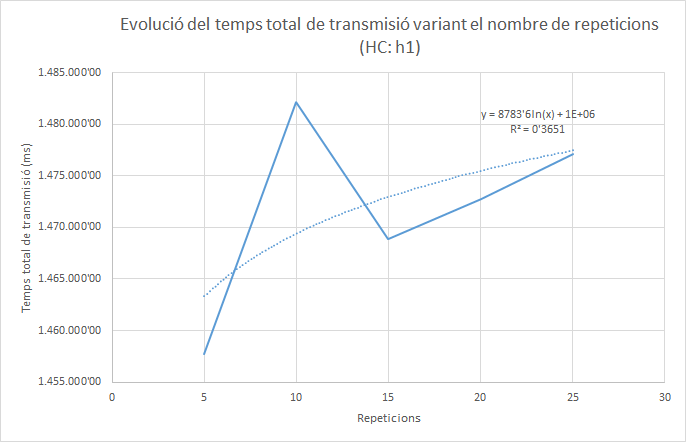
\includegraphics[width=\linewidth]{Exercici7.1.2}
\end{minipage}
\caption{Resultats obtinguts amb l'heurístic 1}
\end{figure}

\begin{figure}[h!]
	\begin{minipage}[b]{0.49\linewidth}
		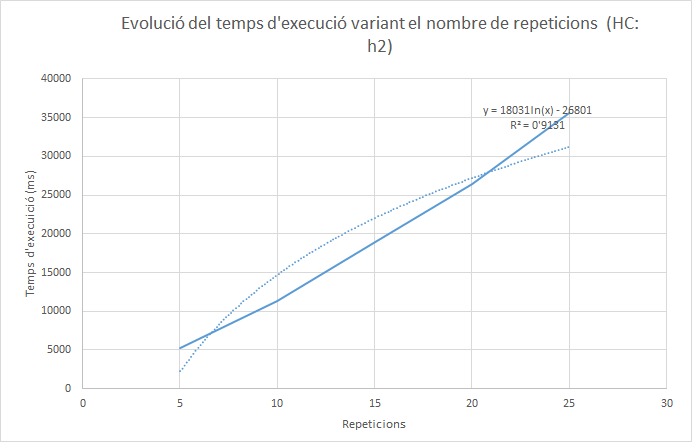
\includegraphics[width=\linewidth]{Exercici7.2.1}
	\end{minipage}
	\begin{minipage}[b]{0.49\linewidth}
		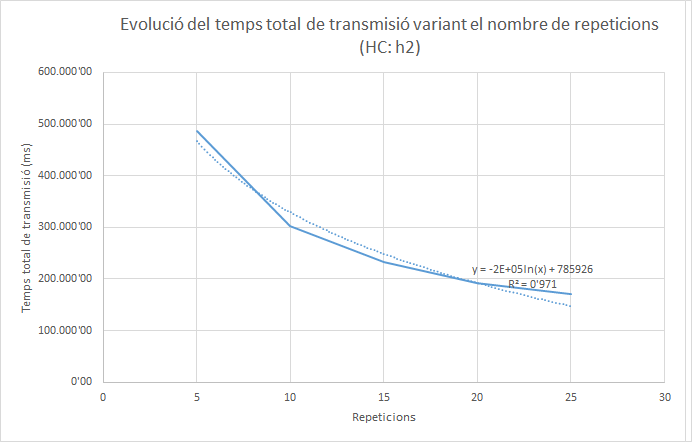
\includegraphics[width=\linewidth]{Exercici7.2.2}
	\end{minipage}
\caption{Resultats obtinguts amb l'heurístic 2}
\end{figure}

\newpage
\subsection{}
En aquest experiment s'ha de fer un anàlisi final dels dos algoritmes, en els experiments anteriors 
es pot veure que el Hill Climbing només troba resultats bons si usa l'heurístic 2, però aquest 
triga molt en trobar les seves solucions. En canvi el Simulated Annealing pot arribar molt ràpidament
a resultats bastant bons, però no tant com els del Hill Climbing amb l'heurístic 2. La decisió entre 
quin dels dos algoritmes triar es basarà en què resulta mes important pel nostre cas. Si es té una alta 
potencia de processament segurament es millor agafar com a algoritme el Hill Climbing amb el segon 
heurístic. En canvi si la potencia de processament es tan baixa que es més perjudicial trigar en trobar 
una solució que tenir-ne una molt poc optima seria millor el Simulated Annealing.

\end{document}